\documentclass[]{article}
\usepackage{polski}
\usepackage[utf8]{inputenc}
\usepackage{amsmath}
\usepackage{graphicx}
\usepackage{caption}
\usepackage{subcaption}
\usepackage{geometry}
\usepackage{float}

\geometry{legalpaper, margin=0.6in}


%opening
\title{TST - Projekt 1}
\author{Jakub Postępski}

\begin{document}

\maketitle


\section{Wprowadzenie}
Przyjmijmy macierz $A_{2x2}$.

Macierz posiada, dla $i = {1, 2}$:
\begin{itemize}
	\item wartości własne $\lambda_i$
	\item wektory własne $\vec{v_i}$ 
\end{itemize}

W zadaniu interesuje nas dynamika ciągu:
\[x^{(t)} = A^tx_0 \]

\section{Wartości własne}

Podstawowym równaniem jest:
\[ Ax = \lambda x\]

Zbiór rozwiązań to widmo: \[\sigma(A) = \{ \lambda_i \in \  \} \]
W ten sposób szukamy wartości dla których macierz $A$ zachowa się jak przekształcenie liniowe (skalar). Dla takich wartości macierz tylko powiększa lub zmniejsza zadany wektor, ale nie zależności pomiędzy składowymi wektora. 

Z równania wynika, że wartości własne decydują o tym jakim przekształceniem będzie macierz $A$.

\section{Wektory własne}
Są wektorami rozpinającymi bazę którą tworzy przekształcenie macierzy A. Zestaw takich wektorów nie jest jednoznaczny. Dla jednej macierzy można znaleźć wiele zestawów wektorów rozpinających. Wektory własne decydują więc o obrocie (konfiguracji) naszego przekształcenia. 

\section{Związek wartości i wektorów własnych}
Wiemy już, że wartości własne (poniżej zapisane w diagonalnej macierzy $D$) definiują przekształcenie, a zestaw wektorów własnych (poniżej zapisane w macierzy $V$) jego obrót. Aby przekształcenie zachowywało się tak samo (pod względem widma) jak $D$ musi zachodzić (szukamy macierzy podobnej):
\[A = VDV^{-1}\]

dzięki czemu jesteśmy w stanie znaleźć macierz $A$.

Ciekawostka której jeszcze nie przemyślałem: Możemy przekształcić do $AV = VD$ i wtedy zbiór wektorów własnych ma jakieśtam wartości własne, które definiują przekształcenie którym działamy na $D$. 

\section{Dynamika układów}
\begin{figure}
	\centering
	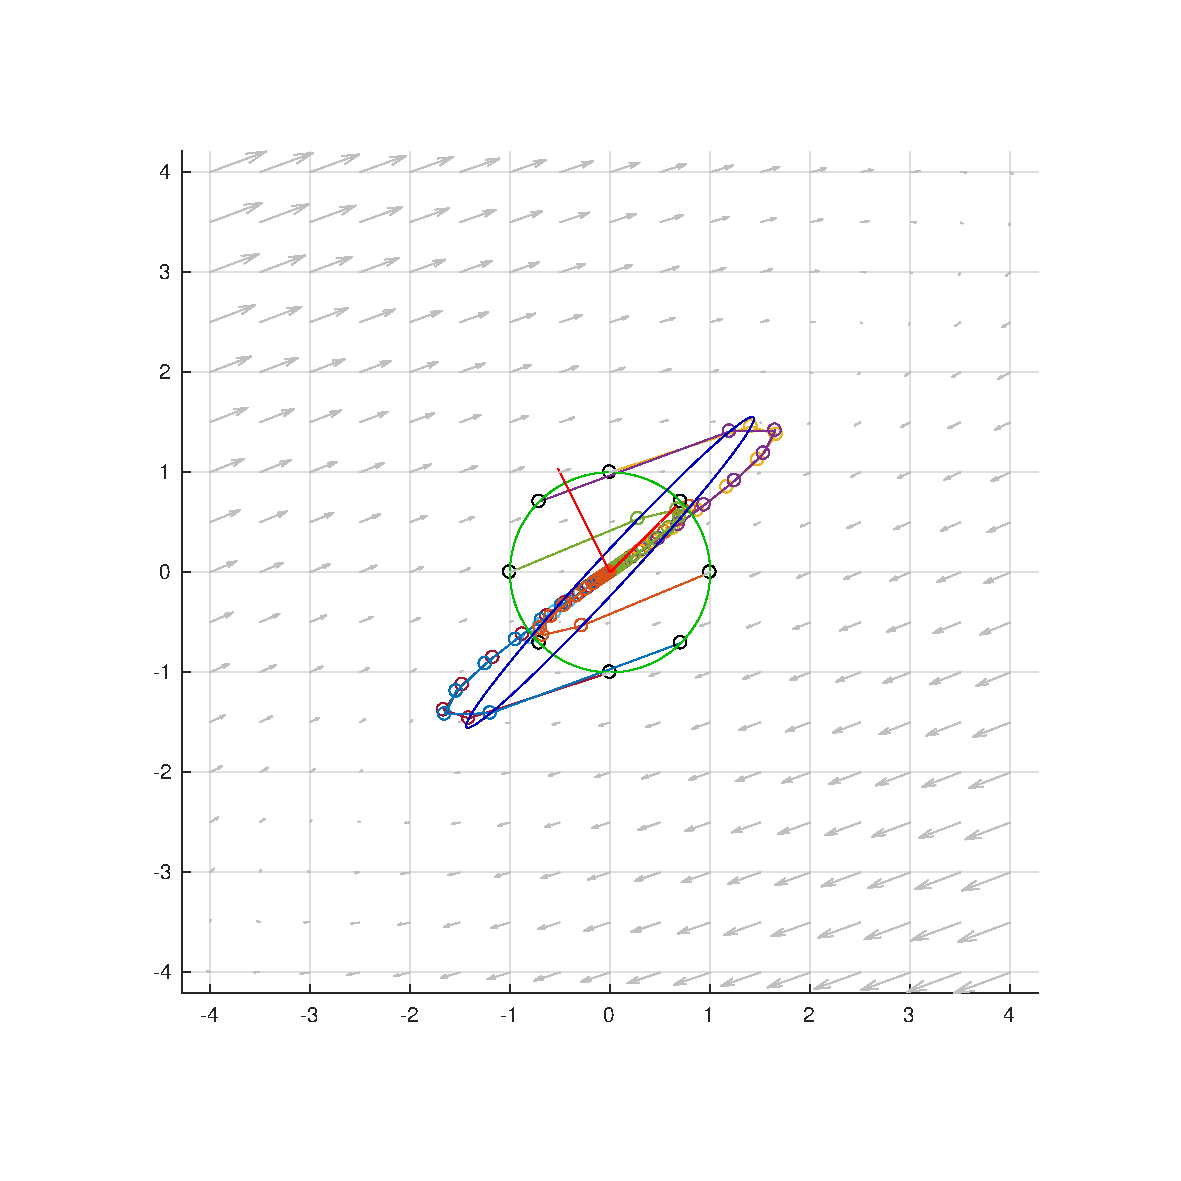
\includegraphics[width=0.99\linewidth]{demo}
	\caption{Przykładowy układ z losowymi wartościami. "Popychany" przez gradient układ zbiega do zera, zgodnie z wyznaczonym obrazem.}
	\label{fig:normal0}
\end{figure}


\begin{figure}
	\centering
 	\begin{subfigure}{.5\textwidth}
		\centering
		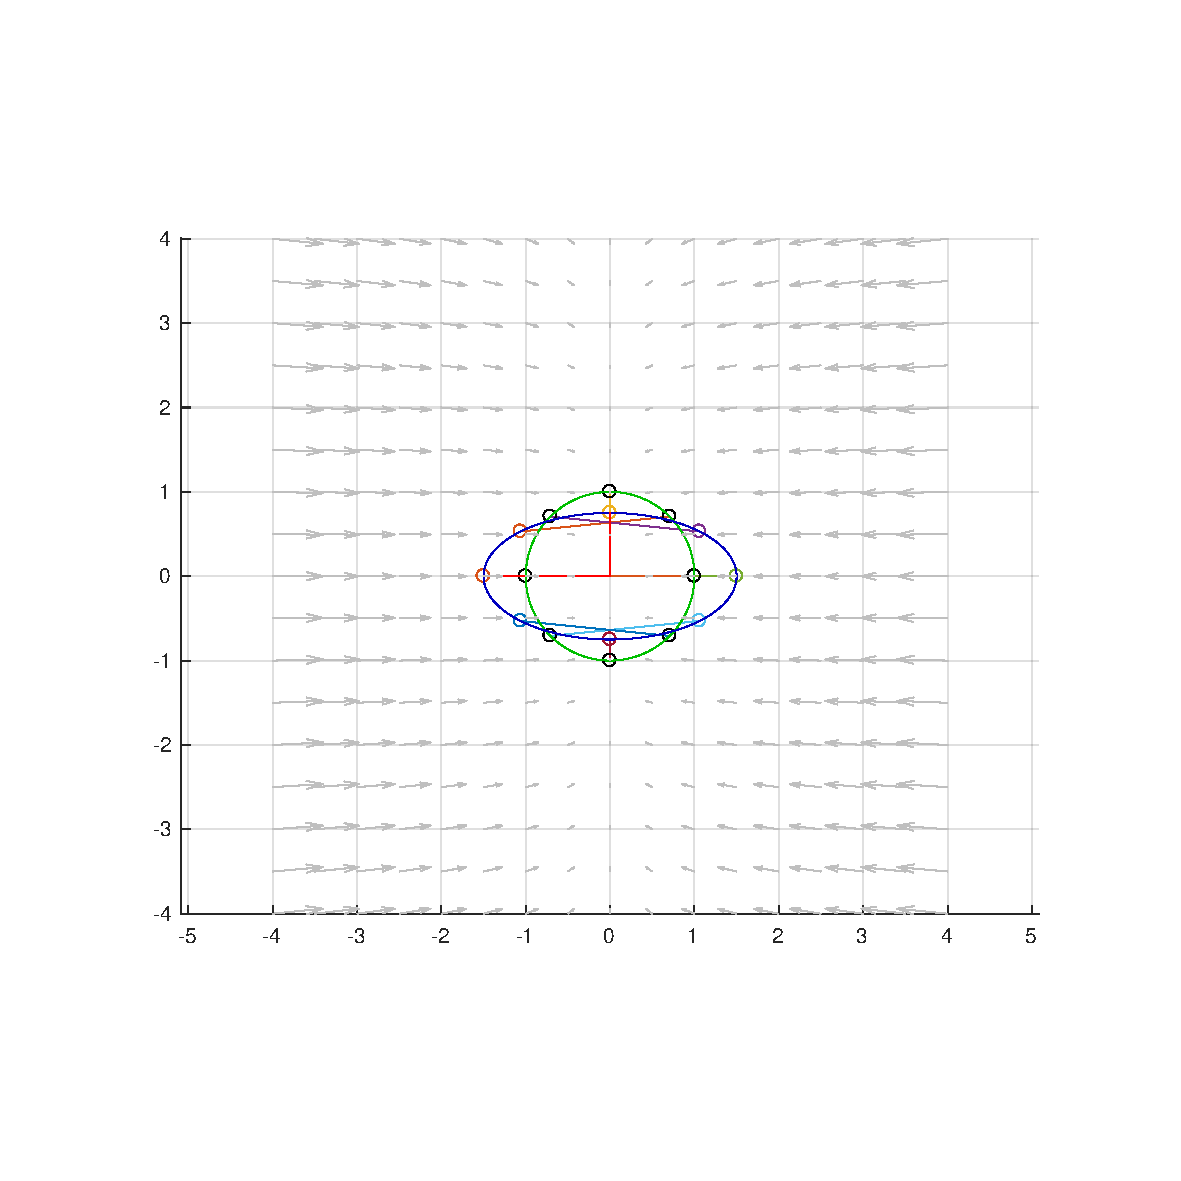
\includegraphics[width=0.99\linewidth]{normal_075_-15}
		\caption{$\lambda_1 = 0.75, \lambda_2 = -1.5$}
		\label{fig:rotation1}
	\end{subfigure}%
	\begin{subfigure}{.5\textwidth}
		\centering
		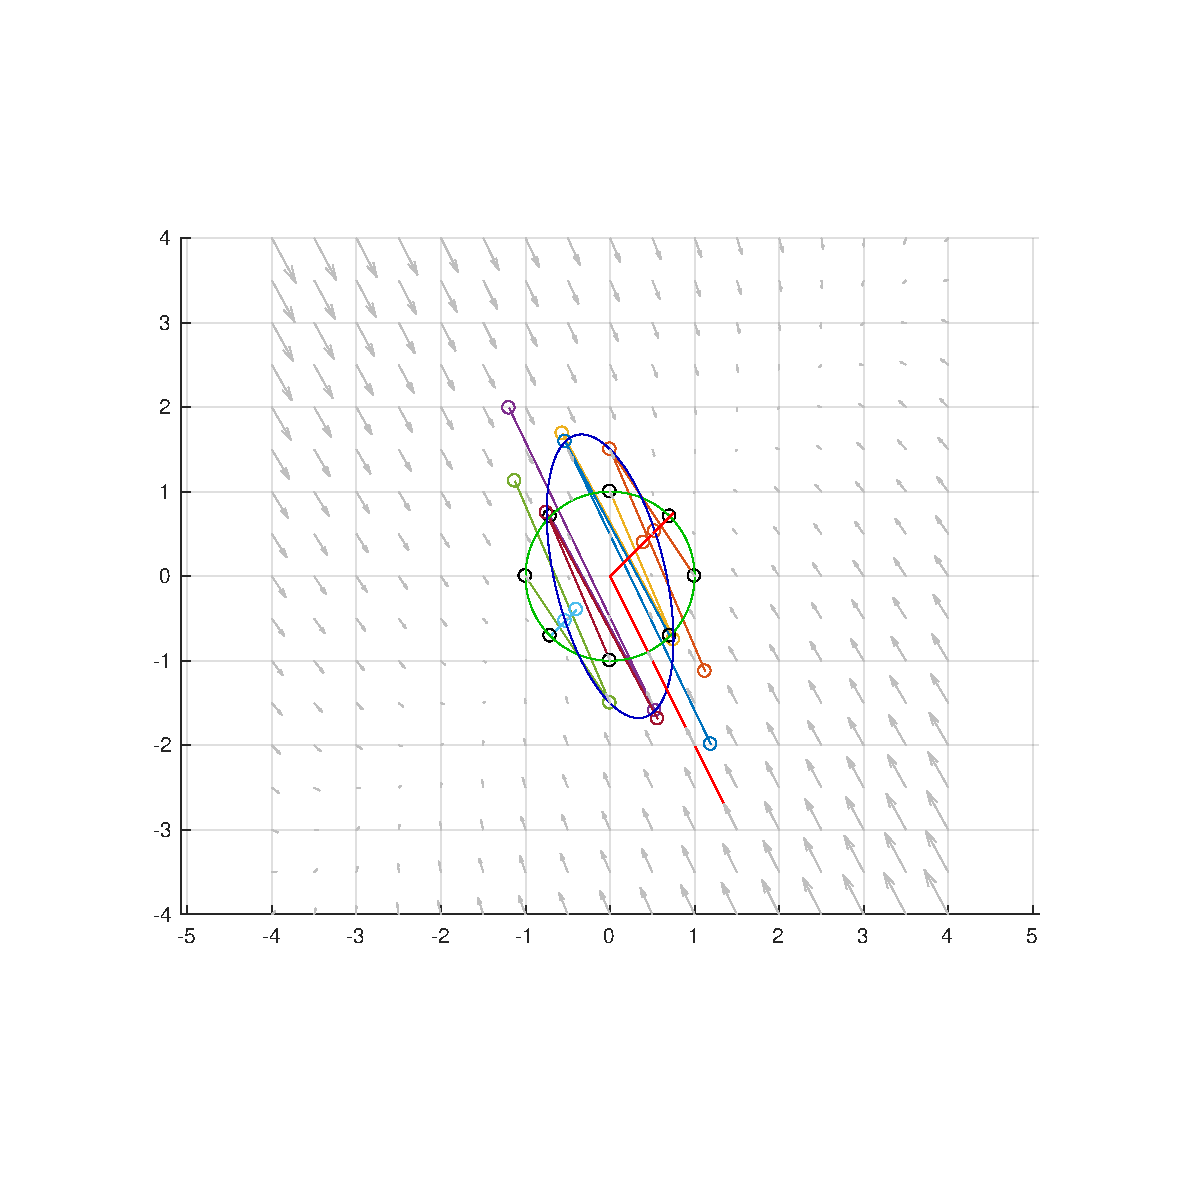
\includegraphics[width=0.99\linewidth]{rotated_075_-15}
		\caption{$\lambda_1 = 0.75, \lambda_2 = -1.5$}
		\label{fig:rotation2}
	\end{subfigure}
	\caption{Porównanie układów z jednakowymi wartościami własnymi. Różne wektory własne powodują obrót i przeskalowanie przekształcenia.}
	\label{fig1}
\end{figure}

\begin{figure}
	\centering
	\begin{subfigure}{.5\textwidth}
		\centering
		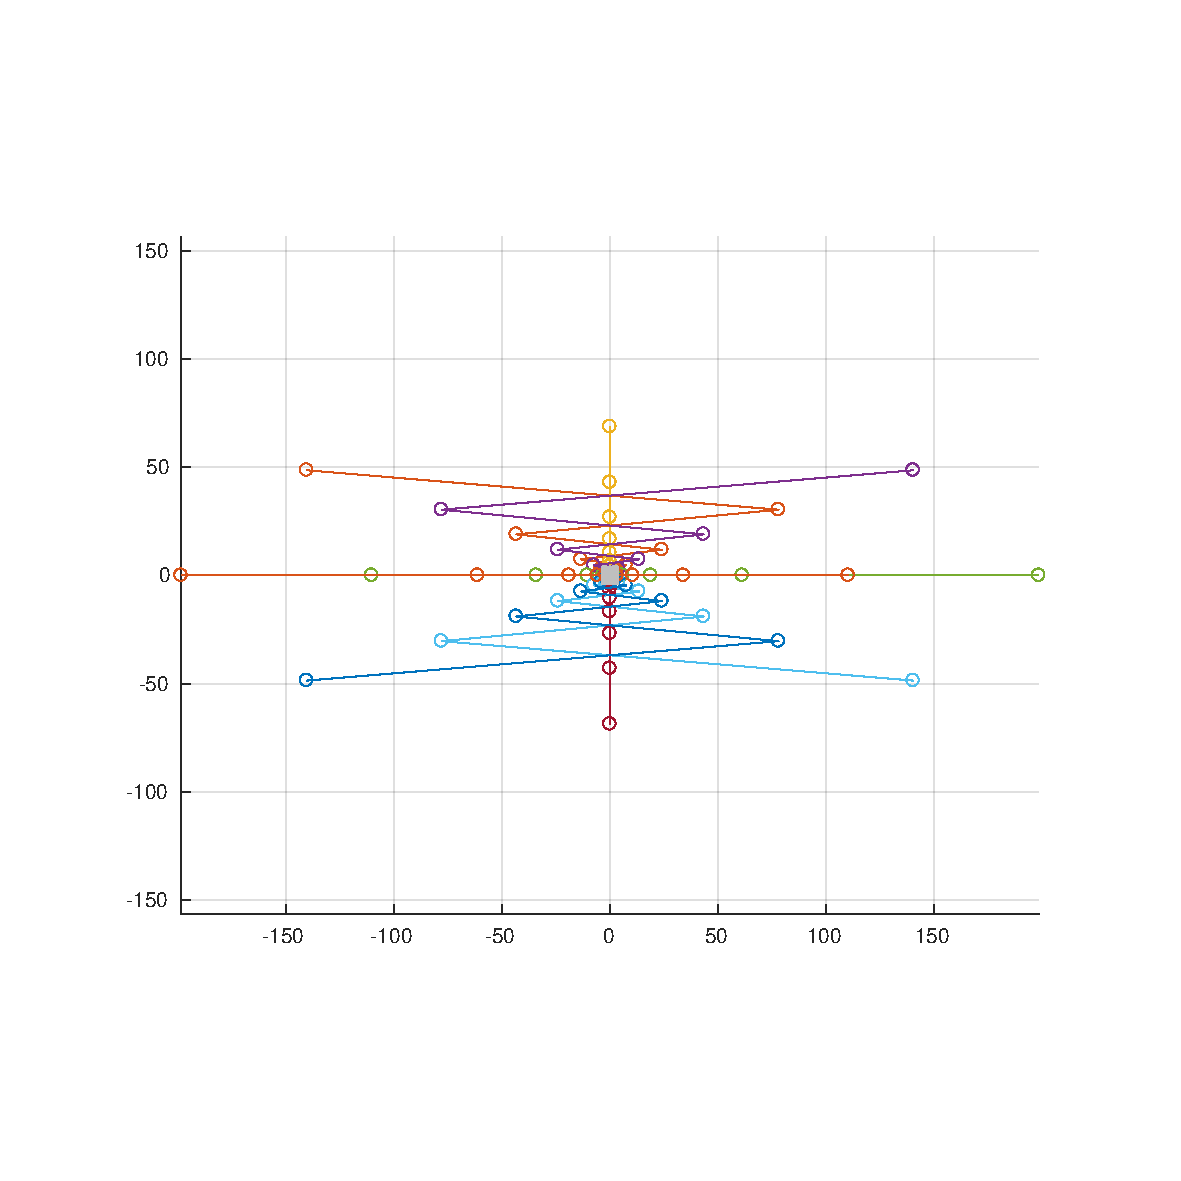
\includegraphics[width=0.99\linewidth]{normal_16_-18}
		\caption{$\lambda_1 = 1.6, \lambda_2 = -1.8$}
		\label{fig:normal1}
	\end{subfigure}%
	\begin{subfigure}{.5\textwidth}
		\centering
		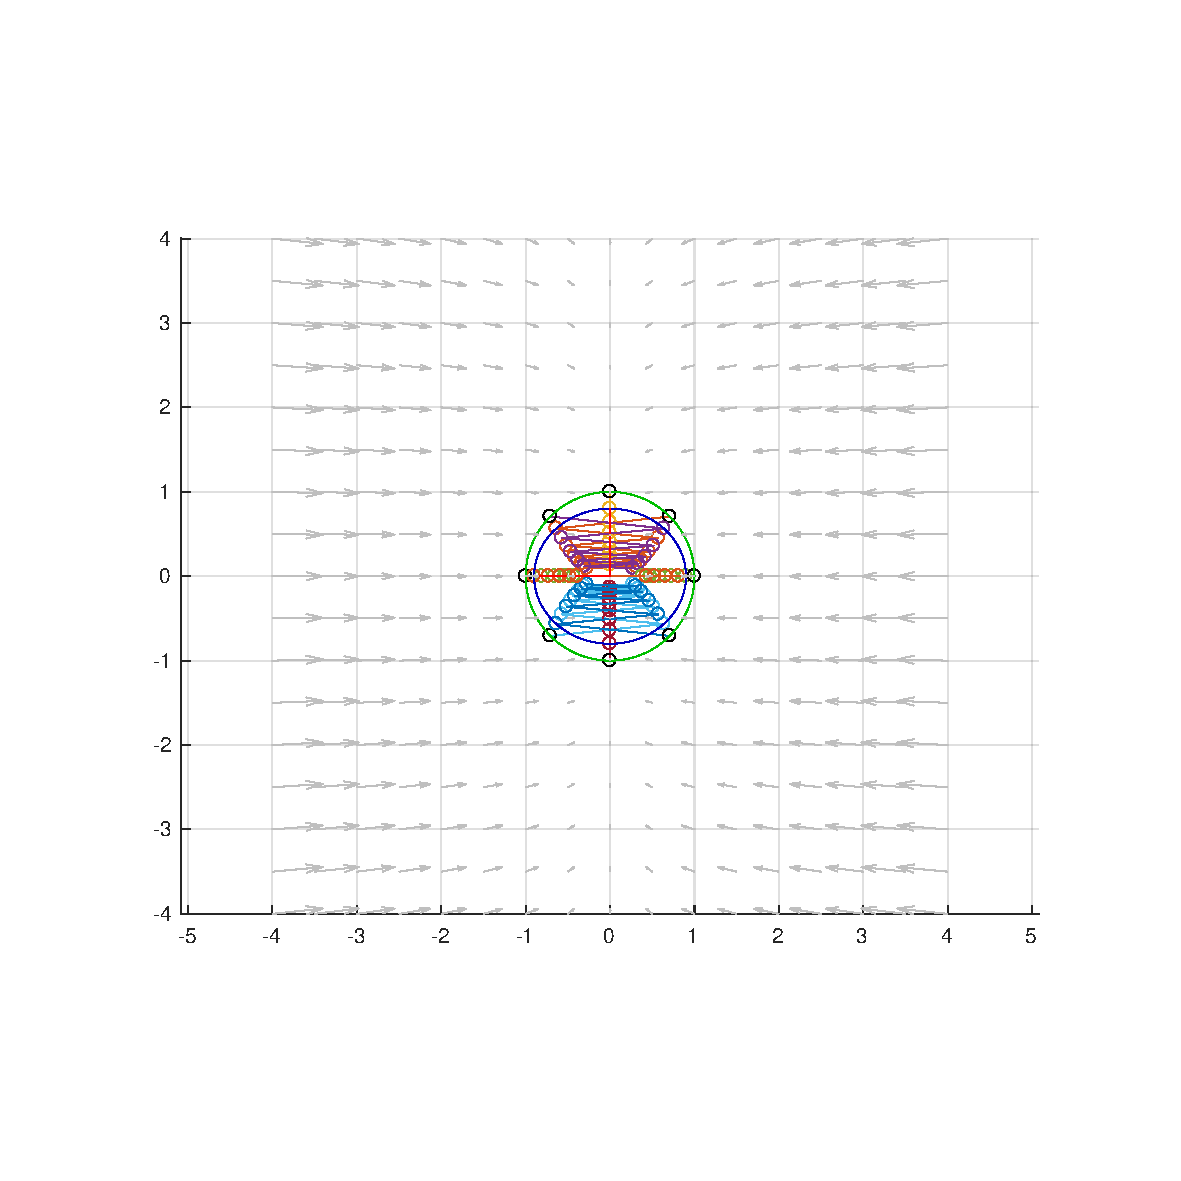
\includegraphics[width=0.99\linewidth]{normal_08_-09}
		\caption{$\lambda_1 = 0.8, \lambda_2 = -0.9$}
		\label{fig:normal2}
	\end{subfigure}
	\caption{Porównanie promieni spektralnych. W drugim przypadku $\rho < 1$. Por.: Układ rozbiega się; Układ zbiega do zera.}
	\label{fig2}
\end{figure}


\begin{figure}
	\centering
	\begin{subfigure}{.5\textwidth}
		\centering
		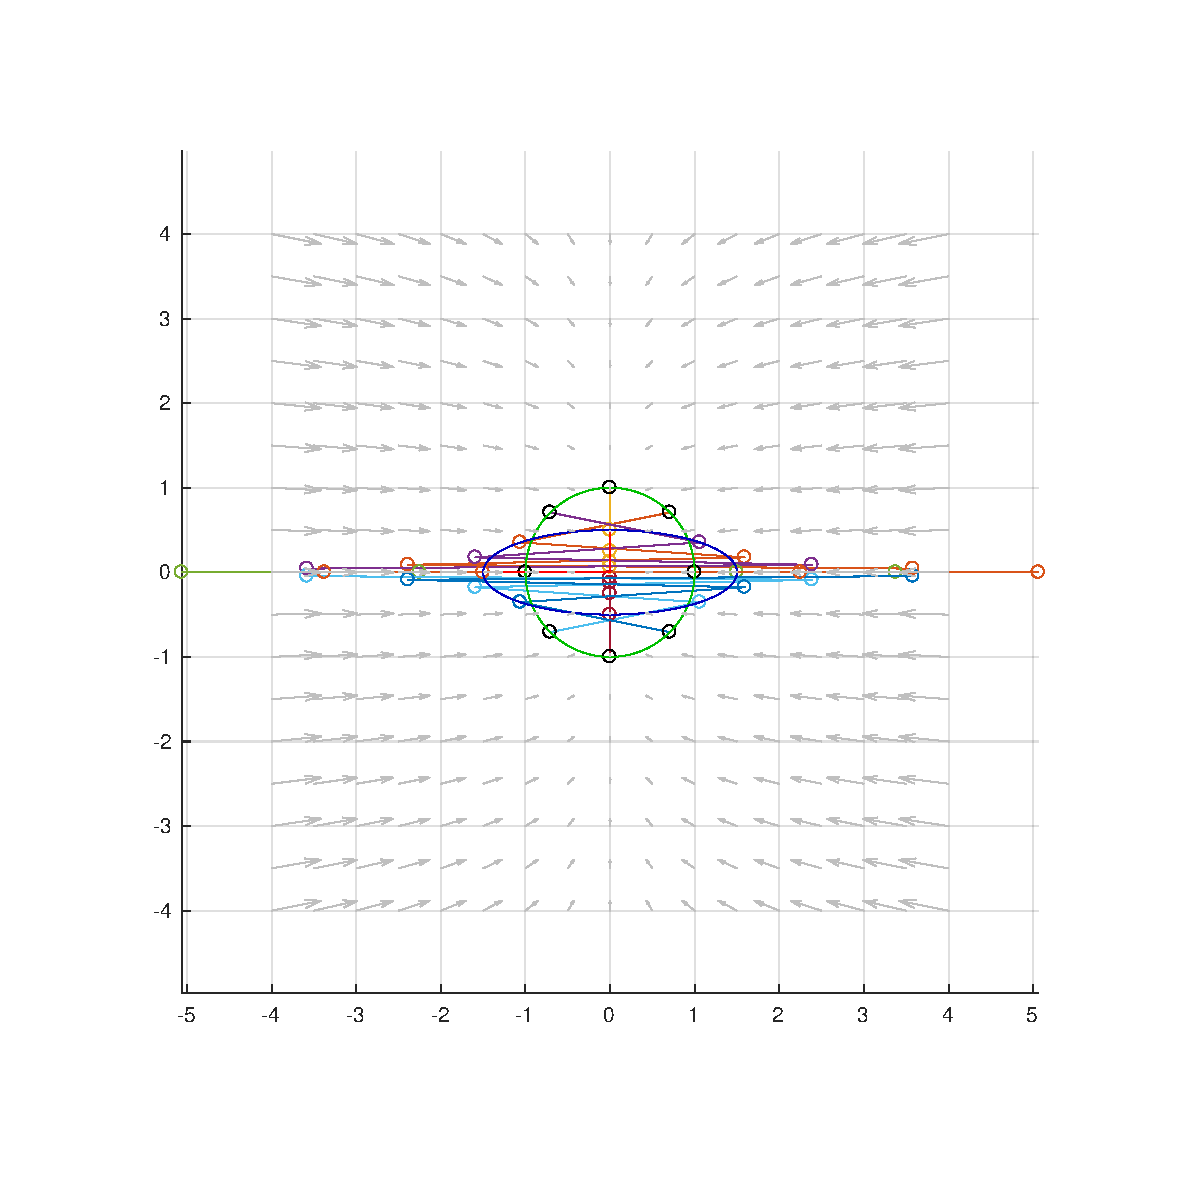
\includegraphics[width=0.99\linewidth]{imag_0-15_05}
		\caption{$\lambda_1 = -1.5, \lambda_2 = 0.5$}
		\label{fig:imag1}
	\end{subfigure}%
	\begin{subfigure}{.5\textwidth}
		\centering
		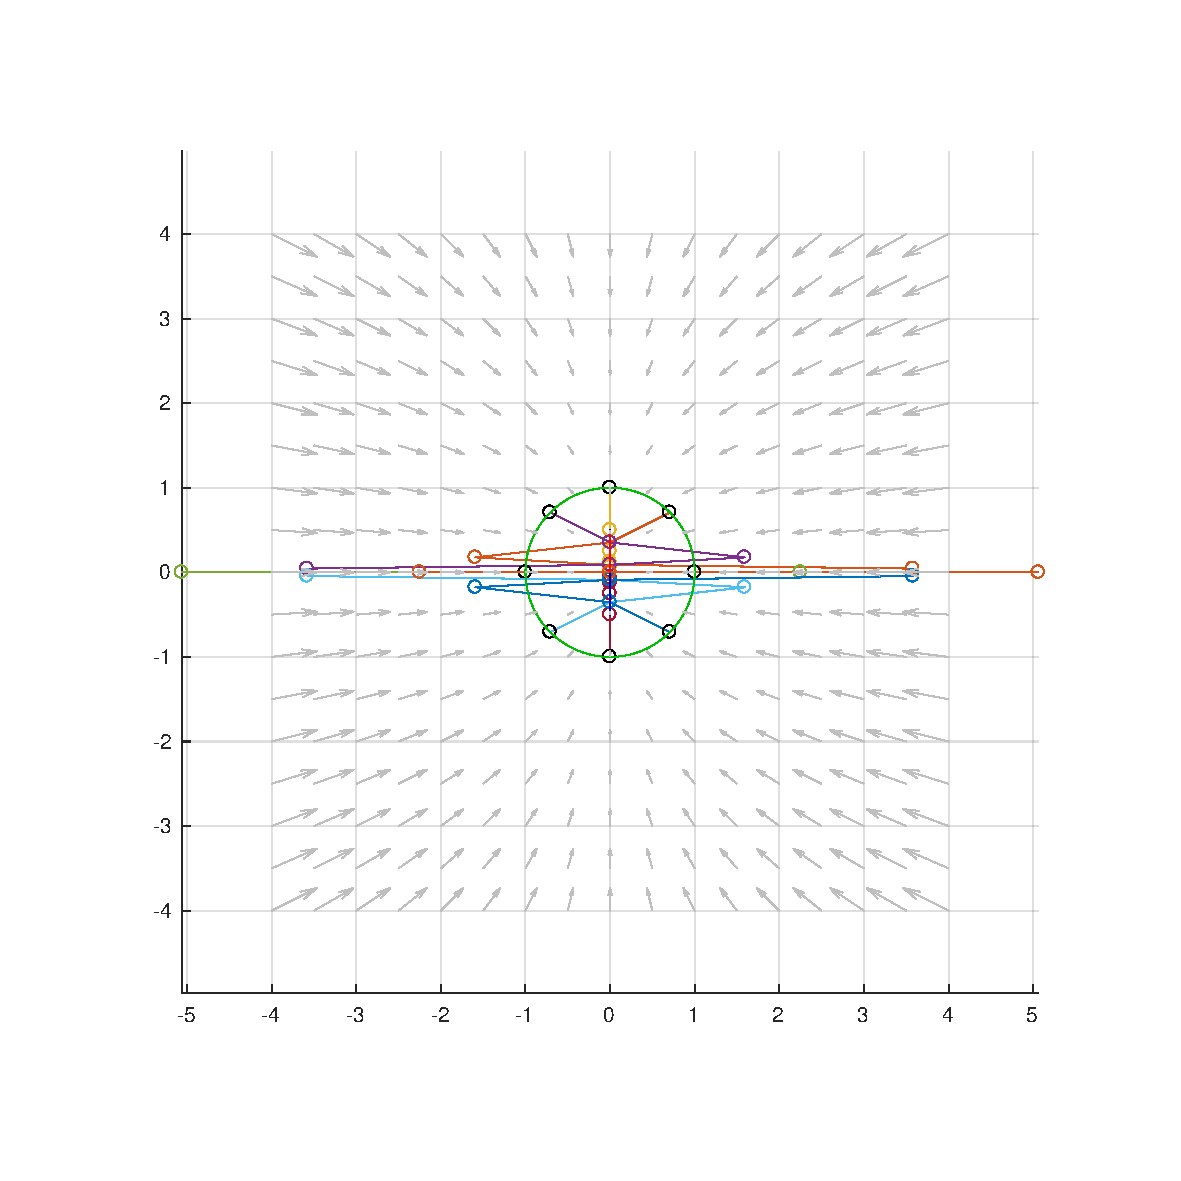
\includegraphics[width=0.99\linewidth]{imag_0-15i_05}
		\caption{$\lambda_1 = -1.5i, \lambda_2 = 0.5$}
		\label{fig:imag2}
	\end{subfigure}
	\caption{Zastosowanie jednego bieguna zespolonego. Por.: Rzutowanie na okrąg; Rzutowanie na prostą.}
	\label{fig3}
\end{figure}

\end{document}
